\documentclass{beamer}
\setbeamertemplate{navigation symbols}{}
\setbeamertemplate{caption}{\insertcaption}

\usetheme{Dresden}
\usecolortheme{beaver}

\usepackage{amsmath}
\graphicspath{{figs/}}
\usepackage{multirow}

\usepackage{tikz}

\let\Tiny\tiny
\usepackage{graphicx}
\usepackage{xmpmulti}
\usepackage{multimedia}
%\usepackage{media9}


\beamersetuncovermixins{\opaqueness<1>{25}}{\opaqueness<2->{15}}

\begin{document}
	\title{Neural Networks}  
	\author{Saumya Bhatnagar}
	\date{\today} 
	
	
\begin{frame}
\titlepage
\end{frame}

\begin{frame}[allowframebreaks]\frametitle{Table of contents}\tableofcontents
\end{frame} 




\section{General}
\begin{frame}
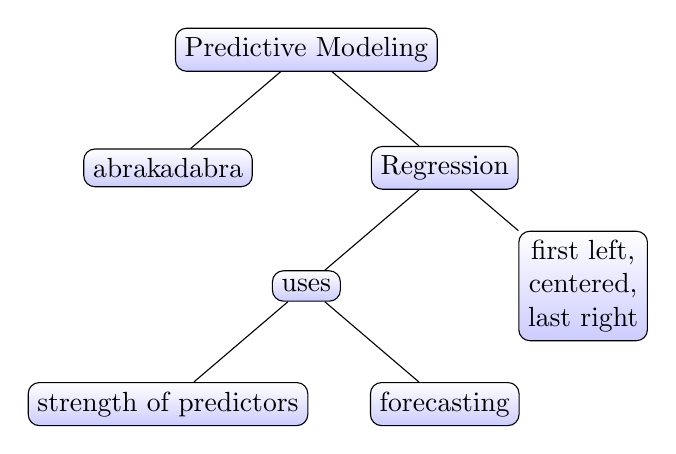
\begin{tikzpicture}[sibling distance=10em,
every node/.style = {shape=rectangle, rounded corners,
	draw, align=center,
	top color=white, bottom color=blue!20}]]
\node {Predictive Modeling}
child { node {abrakadabra} }
child { node {Regression}
	child { node {uses}
		child { node {strength of predictors} }
		child { node {forecasting} }
		%child { node {center} } 
	}
	child { node {first left,\\centered,\\last right} } };
\end{tikzpicture}
\end{frame}

\begin{frame}[plain]%\frametitle{ML}
\begin{columns}
\begin{column}{0.7\textwidth}
	\includegraphics[scale=0.2]{mlinit}\\
	\includegraphics[scale=0.2]{mlmethods}
\end{column}
\begin{column}{0.3\textwidth}
	\includegraphics[scale=0.2]{mlmethods}
\end{column}
\end{columns}
\end{frame}

\begin{frame}[plain]
\hspace*{-3pt}\makebox[\linewidth][c]{

\includegraphics[scale=0.82]{mltypes}
}
\end{frame}


\begin{frame}\frametitle{Why to Study Neural Computation}
	\begin{itemize}
		\item to study how brain works
		\item to understand the styles of parallel computations inspired by neurons and their adaptive connections
		\item to solve practical problems by using novel learning algorithms inspired by brain
	\end{itemize}
\end{frame}



\begin{frame}\frametitle{TIMIT BENCHMARK FOR SOUND}
	content...
\end{frame}


%%%%%%%%%%%%%%%%%%%%%%%%%%%%%%%%%%%%%%%%%%%%%%%%%%%%%%%%%%%%%%%%%%%%%%%%%%%%%%%%%%%%%%%%%%%%%%%%%%%%%%%%%%%%%%%%%%%%%%%%%%%%%%%%%%%%%%%

\subsection{ANN}


\begin{frame}[allowframebreaks]\frametitle{Linear Neurons}
	\begin{columns}
		\begin{column}{0.4\textwidth}
			\textbf{Linear Neurons}\\
			Output, y = b + $\sum x_i w_i$\\
			= activities on input line times weight\\
			$x_i = i^{th}$ input\\
			$w_i = i^{th}$ weight\\
			$b = bias$\\
			
		\end{column}
		\begin{column}{0.7\textwidth}
			\textbf{Binary Threshold Neurons}\\
			\textbf{Output, z = b + $\sum x_i w_i$}
			\begin{align}
			y = \left\{ \begin{array}{cc} 
			1, & \hspace{5mm} z >=0 \\
			0, & \hspace{5mm} otherwise \\
			\end{array} \right.
			\end{align}
			OR Output, z = $\sum x_i w_i$\\
			\begin{align}
			y = \left\{ \begin{array}{cc} 
			1, & \hspace{5mm} z >=\theta \\
			0, & \hspace{5mm} otherwise \\
			\end{array} \right.
			\end{align}

			$\theta$ = threshold = -b
			
		\end{column}
		\end{columns}

	\begin{columns}

		\begin{column}{0.35\textwidth}
			\textbf{Sigmoid Neurons}\\
			Output, z = b + $\sum x_i w_i$\\
			derivatives makes learning easy\\
			use logistic function, y = $\frac{1}{1+se^{-z}}$\\
			\textbf{Stochastic Binary Neurons}: o/p of logistic as probability of spike in a short time window\\
			p(s=1) = $\frac{1}{1+se^{-z}}$\\
			
		\end{column}
		\begin{column}{0.65\textwidth}
			\textbf{Rectified Linear Neurons}\\
			aka Linear Threshold Neurons\\
			Output, z = b + $\sum x_i w_i$\\
			= non-linear function $\leftarrow$ linear weighted sum of inputs 	
			\begin{align}
			y = \left\{ \begin{array}{cc} 
			z, & \hspace{5mm} z >=0 \\
			0, & \hspace{5mm} otherwise \\
			\end{array} \right.
			\end{align}
			\textbf{Apply stochastic methods in ReLU}\\
			o/p = rate of producing spikes (deterministic)\\
			use rate to get the actual times at which spikes are produced $\Rightarrow$ Random process $\Rightarrow$Poisson process\\
			ReLU determines the rate but intrinsic randomness in unit determines when the spikes are actually produced
		\end{column}
	\end{columns}




	\includegraphics[scale=0.265]{DNN/activationf}
	\includegraphics[scale=0.22]{DNN/activationfuses}

\end{frame}


\begin{frame}\frametitle{Supervised vs Unsupervised vs Reinforcement Learning}
	Model-class: Predicted output, $\hat{y} = f(x;W)$\\
	W = Numerical parameters\\
	input vector\\
	Regression, minimize $\frac{1}{2}(y-\hat{y})^2$\\
	\textbf{Reinforcement Learning:}\\
	o/p is action or sequence of actions\\
	supervision by rewards\\
	max expected sum of future rewards\\
	use discount factor for delayed rewards, so won't have to look too far into future\\
	\textbf{why not RL?}: in long sequence of actions rewards are delayed so it's hard to know where we went wrong\\
	a scalar reward doesn't supply much info
\end{frame}

\begin{frame}\frametitle{Feedforward NN}
	information comes from input unit, flows in one direction towards hidden layer and gives the output\\
	if more than one hidden layer $\Rightarrow$ \textbf{Deep NN}\\
	compute transformations:\\
	activities of neurons in each layer are a  non-linear func of the activities in layer below\\
	
\end{frame}

\begin{frame}\frametitle{Perceptron convergence procedure}
	training binary o/p neurons as classifiers\\
	add an extra component with value 1 to each i/p vector. the "bias" wt on this component is minus the threshold. now forget the threshold.\\
	pick training cases using any policy that ensures that every training case will keep getting picked\\
	\begin{itemize}
		\item if o/p is correct, do nothing
		\item if incorrectly o/ps to 0, add i/p vector to wt vector
		\item if incorrectly o/ps to 1, subtract i/p vector from wt vector
	\end{itemize}

\end{frame}

\begin{frame}\frametitle{Padding and stride}
	\textbf{Padding }is used to preserve the boundary information , since without padding they are only traversed once.//

\end{frame}

\begin{frame}\frametitle{example}
content...
\end{frame}









%%%%%%%%%%%%%%%%%%%%%%%%%%%%%%%%%%%%%%%%%%%%%%%%%%%%%%%%%%%%%%%%%%%%%%5
\subsection{RNN}


\begin{frame}
	Sequential Data\\
	o/p dependent on prev computations saved in memory\\
	\textbf{Feedforward}(touches node once) vs \textbf{RNN}(loops: present in recent past)\\
	why not feedforward?: can't predict the next word in a sentence if I use feed-forward\\
	Backpropagation of error and gradient descent\\
	Error will return via \textbf{Backpropagation} adjusting weights\\
	sentence of 5 words, 5 layered NN\\
	\begin{itemize}
		\item $\sim$ very deep nets with hidden layer per time slice
		\item get input at every time slice
		\item use same weights at every time slice
	\end{itemize}

RNN with multiple hidden layers are special case where some hidden $\rightarrow$ hidden connections are missing

\end{frame}

\begin{frame}\frametitle{}
	content...
\end{frame}


\subsection{CNN}

\begin{frame}[allowframebreaks]\frametitle{convnets}
	A convolution operation is basically computing a dot product between their weights and a small region they are connected(currently overlapping) to in the input volume. This will change the dimensions depending on the filter size used and number of filters used.\\
	Each neuron receives some inputs, performs a dot product and optionally follows it with a non-linearity.\\
	\includegraphics[scale=0.4]{CNN/structure}\\
	a loss function (e.g. SVM/Softmax) on the last (fully-connected) layer\\
\end{frame}



\begin{frame}\frametitle{spatial size of the output volume}
	for calculating how many neurons "fit", use\\
	(W-F+2P)/S + 1\\
	is a function of the:\\
	input volume size (W),\\
	the receptive field size of the Conv Layer neurons (F), \\
	the stride with which they are applied (S), \\
	and the amount of zero padding used (P) on the border\\
	For example for a 7x7 input and a 3x3 filter with stride 1 and pad 0 we would get a 5x5 output. With stride 2 we would get a 3x3 output.

\end{frame}


\section{Optimization}

\begin{frame}\frametitle{Non-Linear Optimization}
	
\end{frame}


\section{Graph Theory}


\section{Algorithms \& Data Structures}
\begin{frame}\frametitle{OOPS}
	Overloading vs overriding
\end{frame}

\begin{frame}\frametitle{Abstract vs Interface}
	content...
\end{frame}

\begin{frame}\frametitle{Principle}
	\textbf{ACID}: Atomic ... Isolate ...\\
	\textbf{Dependency Inversion Principle}: High level module shouldn't depend on low level module\\
	\textbf{Liskov Principle}\\
	Interface segregation\\
	CURD (Create, Read, Update, Delete)\\
\end{frame}


\begin{frame}\frametitle{Non}
	content...
\end{frame}


\section{Autoencoders}


\section{RBM - Restrictive Boltzmann Machine}






\begin{frame}
	Thank You!
\end{frame}

\end{document}